\documentclass{article}
%\usepackage[a4paper,margin=2.2cm,footskip=.5cm]{geometry}
\usepackage{fullpage}
%-----------------Hyperlink Packages--------------------
\usepackage{hyperref}
\hypersetup{
	 colorlinks   = true,
     citecolor    = black,
     linkcolor    = black,
     urlcolor     = black
}
%-----------------Figure Packages--------------------
\usepackage{graphicx}                       % For figures
\usepackage{stfloats}
\usepackage{caption}
\usepackage[export]{adjustbox}
\usepackage[tight,footnotesize]{subfigure}  % Create subfigures, ie 1A, 1B
%\usepackage{epsfig} % for postscript graphics files
%------------------Math Packages------------------------
\usepackage{amssymb,amsmath}
\usepackage{textcomp}
\usepackage{mdwmath}
\usepackage{mdwtab}
\usepackage{eqparbox}
%------------------Table Packages-----------------------
\usepackage{rotating}                     % Used to rotate tables
\usepackage{array}                        % Fixed column widths for tables
%-----------------Algorithm Packages--------------------
\usepackage{listings}                     % Source code
\usepackage{algorithm}                    % Pseudo Code
\usepackage[noend]{algpseudocode}
%---------------------------------------------------------

\begin{document}

\title {
	DIP Final Project \\
	Haze Removal
}

\author {
	Qiuyi Zhang 12330402 \\
	\href{mailto:joyeec9h3@gmail.com}{joyeec9h3@gmail.com}
}

\date {
	\today
}

\maketitle
\tableofcontents


\section{Introduction}

\subsection{Haze Removal Using Dark Channel Prior}
In computer vision and computer graphics, the formation of a hazy image is usually described by the following model:

$$
\mathbf{I}(\mathbf{x}) = \mathbf{J}(\mathbf{x})t(\mathbf{x}) + \mathbf{A}(1 - t(\mathbf{x}))
$$

where $\mathbf{I}$ is the observed intensity, $\mathbf{J}$ is the scene radiance, $\mathbf{A}$ is the global atmospheric light, and $t$ is the medium transmission. With this model, the goal of haze removal is to recover $\mathbf{J}$, $\mathbf{A}$, and $t$ when $\mathbf{I}$ is given.

In \cite{he2009single}, He proposed an approach to use the dark channel prior for haze removal. For an image $\mathbf{J}$, the dark channel of $\mathbf{J}$ is defined as

$$
J^{dark}(\mathbf{x}) = min_{c \in \{r,g,b\}}( min_{\mathbf{y} \in \Omega(\mathbf{x})}(J^c(\mathbf{y})))
$$

When $\mathbf{J}$ is a haze-free outdoor image, the intensity of $J^{dark}$ in the non-sky region is close to zero. Using this prior, the transmission can be estimated by:

$$
\tilde{t}(\mathbf{x}) = 1 - \omega min_{c}( min_{\mathbf{y} \in \Omega(\mathbf{x})}(\frac{I^c(\mathbf{y})}{A^c}))
$$

where $\omega \in (0, 1]$ is a constant parameter for keeping a certain amount of haze to make the output more natural Here $min_{c}( min_{\mathbf{y} \in \Omega(\mathbf{x})}(\frac{I^c(\mathbf{y})}{A^c}))$ is actually the dark channel of the normalized haze image $\frac{I^c(\mathbf{y})}{A^c}$.

To automatically obtain $\mathbf{A}$ from the input image, we can first pick the top $p\%$ brightest pixels in the dark channel, then, for each color channel, we chose the one with the highest intensity in the input image $\mathbf{I}$ as its atmospheric light.

Now that we have $\tilde{t}(\mathbf{x})$, $\mathbf{A}$ and $\mathbf{I}$, we can recover the haze-free image with:

$$
\mathbf{J}(\mathbf{x}) = \frac{\mathbf{I}(\mathbf{x}) - \mathbf{A}}{max(\tilde{t}(\mathbf{x}),t_0)} + \mathbf{A}
$$

where $t_0$ is a lower bound for $t$ to preserve a certain amount of haze in dense haze regions.

\subsection{Guided filter}

Since a transmission map is just an alpha map, we can apply soft matting to refine the estimated transmission. An efficient approach, as proposed in \cite{he2010guided}, is to use the input image $\mathbf{I}$ to guide the filter $\tilde{t}(\mathbf{x})$.

Define $q$ as a linear transform of a color image $\mathbf{I}$ in a window $\omega_k$ with radius $r$ centered at the pixel $k$:

$$
q_i = \mathbf{a}_k^T\mathbf{I}_i + b_k, \forall i \in \omega_k
$$

where $\mathbf{I}_k$ is a $3 \times 1$ color vector, $\mathbf{a}_k$ is a $3 \times 1$ coefficient vector, $b_k$ is a scalar coefficient. For a filter $p$, the coefficients $\mathbf{a}$ and $b$ can be computed with:

\begin{align*}
\mathbf{a}_k &= (\Sigma_k + \epsilon U)^{-1}(\frac{1}{|\omega|}\sum_{i \in \omega_k}\mathbf{I}_i p_i - \mu_k \bar{p}_k) \\
b_k &= \bar{p}_k - \mathbf{a}_k^T\mu_k \\
q_i &= \bar{\mathbf{a}}_i^T\mathbf{I}_i + \bar{b}_i
\end{align*}

where $\Sigma_k$ is the covariance matrix of $\mathbf{I}$ in $\omega_k$, $\epsilon$ is regularization parameter preventing $\mathbf{a}_k$ from being too large, $U$ is the $3 \times 3$ identity matrix, $\mu_k$ is the mean of $\mathbf{I}$ in $\omega_k$, $|\omega|$ is the number of pixels in $\omega_k$, and $\bar{p}_k$ is the mean of $p$ in $\omega_k$. Then, the resulting $q$ is the desired filter under the guidance of $\mathbf{I}$.

\section{Implementation}

Algorithm~\ref{alg:hr} describes how to remove the haze from the image using the dark channel prior. To refine the transmission map, we implement Algorithm~\ref{alg:gf}.

\begin{algorithm}[H]
\centering
\caption{Haze Removal Using Dark Channel Prior}
\label{alg:hr}
  \begin{algorithmic}[1]
    \Function{Dehaze}{$\mathbf{I}$, $t_{min}$, $A_{max}$, $w$, $p$, $\omega$, $r$, $\epsilon$}
        \Comment{$\mathbf{I}$ is the hazy image}
        \State Compute $\mathbf{I}^{dark}$ with $\mathbf{I}^{dark}(\mathbf{x}) = min_{c \in \{r,g,b\}}( min_{\mathbf{y} \in \Omega(\mathbf{x})}(I^c(\mathbf{y})))$
        \State Find the indexes $\mathbf{D}$ for highest $p\%$  pixels in $\mathbf{I}^{dark}$
        \State Compute atmosphere light $\mathbf{A}$ with $\mathbf{A}_c = max_{\mathbf{d} \in  \mathbf{D}}(\mathbf{I}_c(\mathbf{d}))$
        \State Threshold $\mathbf{A}$ with $A_{max}$
        \State Estimate transmission $\tilde{t}$ with $\tilde{t}(\mathbf{x}) \gets 1 - \omega min_{c}( min_{\mathbf{y} \in \Omega(\mathbf{x})}(\frac{I^c(\mathbf{y})}{A^c}))$
        \State $\tilde{t} \gets$ \Call{Guided Filter}{$\mathbf{I}$, $\tilde{t}$, $r$, $\epsilon$}
        \State Recover $\mathbf{J}$ with $\mathbf{J}(\mathbf{x}) = \frac{\mathbf{I}(\mathbf{x}) - \mathbf{A}}{max(\tilde{t}(\mathbf{x}),t_0)} + \mathbf{A}$
      \State \Return $\mathbf{J}$
    \EndFunction
  \end{algorithmic}
\end{algorithm}

\begin{algorithm}[H]
\centering
\caption{Guided Filter}
\label{alg:gf}
  \begin{algorithmic}[1]
    \Function{Guided Filter}{$\mathbf{I}$, $p$, $r$, $\epsilon$}
        \For{each pixel $k$ in $p$}
	        \State $\omega_k$ is the window with radius $r$ for pixel $k$
	        \State Compute $\Sigma_k$, the convariance matrix of $\mathbf{I}$ in $\omega_k$
	        \State Compute $|\omega|$, the number of pixels in $omega_k$
	        \State Compute $\mu_k$, the mean of $\mathbf{I}$ in $\omega_k$ 
	        \State Compute $\bar{p}_k$, the mean of $p$ in $\omega_k$
	        \State $\mathbf{a}_k = (\Sigma_k + \epsilon U)^{-1}(\frac{1}{|\omega|}\sum_{i \in \omega_k}\mathbf{I}_i p_i - \mu_k \bar{p}_k)$
	        \State $b_k = \bar{p}_k - \mathbf{a}_k^T\mu_k$
	        \State $q_k = \bar{\mathbf{a}}_k^T\mathbf{I}_k + \bar{b}_k$
        \EndFor
      \Return $\mathbf{q}$
    \EndFunction
  \end{algorithmic}
\end{algorithm}


\section{Results and Analysis}

The results in Figure~\ref{fig:result1} -~\ref{fig:result4} are generated with $t_{min} = 0.2, A_{max} = 220, w = 15, p=0.1, \omega=0.95,r=40, \epsilon=10^{-3}$. From top to bottom are the input hazy image, the dark channel, the estimated transmission map, the refined transmission map, the image dehazed with raw transmission map, and the image dehazed with refined transmission map.

From the results, it is easy to see that this approach can remove most of the haze in the image. The refined transmission map, however, can lead to much better results than the raw estimates.

Since generating the dark channel is somewhat similar to applying a min filter to the image, areas with low intensity in the dark channel will greatly affect its neighboring pixels. Therefore, when there are drastic transitions in the dark channel (e.g. between the sky/fog and salient objects), the area with low intensities will ``expand''. For example, in Figure~\ref{fig:result1}, the twigs in the dark channel of the forest are much thicker than in the original image. The leaves with good visibility in the front have low values in the dark channel, resulting in those small squares (usually with the same size as the window) in the dark channel map. Since the raw transmission map is actually calculated with the dark channel of the normalized image, this effect directly leads to the translucent borders around the twigs in the image dehazed with this raw estimate. Other images with this kind of drastic transitions in the dark channel also have the same problems. For example, the distant cones in the second image and the leaves in the last image of Figure~\ref{fig:result1}, the tall buildings in the first three images of Figure~\ref{fig:result2}, the roofs in the first image and the trunk in the second image of Figure~\ref{fig:result3}, etc. all have this kind of borders around them.

From the results it is obvious to see that after guiding the transmission map with the original image, the refined transmission map preserves much more detail than the raw estimate. Most objects become distinguishable in this refined map, and the edges in the tranmission map are closer to those in the original image. Therefore, the images dehazed with this refined transmission map no longer have the weird borders as in those dehazed with the raw estimate.

Since the haze will usually increase the brightness of the image (because they are usually white or gray-ish), the images with a large amount of haze will become relatively darker after dehazing, e.g. the first image in Figure~\ref{fig:result1}, the first two images in Figure~\ref{fig:result2},  the last image in Figure~\ref{fig:result4}. The images with just a thin layer of haze will have a better contrast after dehazing, e.g. the fourth image in Figure~\ref{fig:result1}, the fourth image in Figure~\ref{fig:result2}, the second and the third image in Figure~\ref{fig:result3}, and the first image in Figure~\ref{fig:result4}

During the experiment, we discover that the choice of parameters is crutial in the quality of haze removal. When there are sky regions in the image, $\mathbf{A}$ tends to be large. In this case, we need a higher $t_{min}$ or lower $A_{min}$ to threshold the computation so as to restrict the recovered $\mathbf{J}$ in a reasonable range. To make the guidance more accurate, $r$ should be larger than $w/2$. Larger $r$ can lead to better results, but it will also slow down the process.

\begin{figure}[H]
    \centering
    \begin{minipage}[b]{\linewidth}
        \centering
        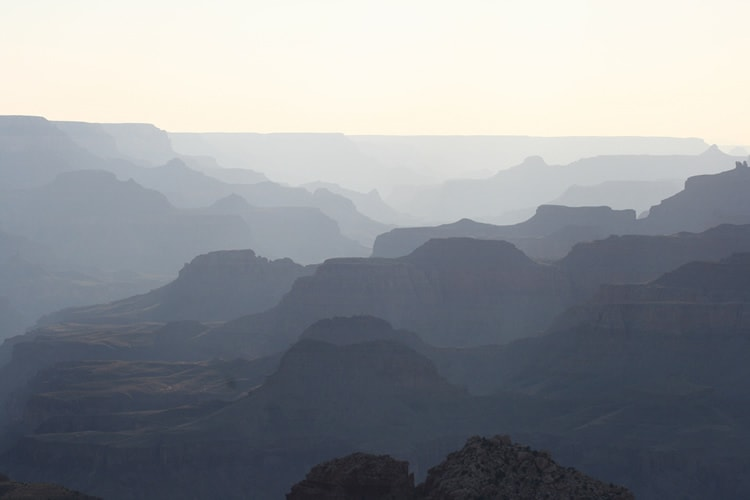
\includegraphics[height=0.18\linewidth]{../img/canon7.jpg}
        \includegraphics[height=0.18\linewidth]{../img/cones.jpg}
        \includegraphics[height=0.18\linewidth]{../img/forest.jpg}
        \includegraphics[height=0.18\linewidth]{../img/flag.jpg}
        \includegraphics[height=0.18\linewidth]{../img/house-input.png}
    \end{minipage}
    \begin{minipage}[b]{\linewidth}
        \centering
        \includegraphics[height=0.18\linewidth]{../result/canon7-dark.jpg}
        \includegraphics[height=0.18\linewidth]{../result/cones-dark.jpg}
        \includegraphics[height=0.18\linewidth]{../result/forest-dark.jpg}
        \includegraphics[height=0.18\linewidth]{../result/flag-dark.jpg}
        \includegraphics[height=0.18\linewidth]{../result/house-input-dark.png}
    \end{minipage}
    \begin{minipage}[b]{\linewidth}
        \centering
        \includegraphics[height=0.18\linewidth]{../result/canon7-rawt.jpg}
        \includegraphics[height=0.18\linewidth]{../result/cones-rawt.jpg}
        \includegraphics[height=0.18\linewidth]{../result/forest-rawt.jpg}
        \includegraphics[height=0.18\linewidth]{../result/flag-rawt.jpg}
        \includegraphics[height=0.18\linewidth]{../result/house-input-rawt.png}
    \end{minipage}
    \begin{minipage}[b]{\linewidth}
        \centering
        \includegraphics[height=0.18\linewidth]{../result/canon7-refinedt.jpg}
        \includegraphics[height=0.18\linewidth]{../result/cones-refinedt.jpg}
        \includegraphics[height=0.18\linewidth]{../result/forest-refinedt.jpg}
        \includegraphics[height=0.18\linewidth]{../result/flag-refinedt.jpg}
        \includegraphics[height=0.18\linewidth]{../result/house-input-refinedt.png}
    \end{minipage}
    \begin{minipage}[b]{\linewidth}
        \centering
        \includegraphics[height=0.18\linewidth]{../result/canon7-radiance-rawt.jpg}
        \includegraphics[height=0.18\linewidth]{../result/cones-radiance-rawt.jpg}
        \includegraphics[height=0.18\linewidth]{../result/forest-radiance-rawt.jpg}
        \includegraphics[height=0.18\linewidth]{../result/flag-radiance-rawt.jpg}
        \includegraphics[height=0.18\linewidth]{../result/house-input-radiance-rawt.png}
    \end{minipage}
    \begin{minipage}[b]{\linewidth}
        \centering
        \includegraphics[height=0.18\linewidth]{../result/canon7-radiance-refinedt.jpg}
        \includegraphics[height=0.18\linewidth]{../result/cones-radiance-refinedt.jpg}
        \includegraphics[height=0.18\linewidth]{../result/forest-radiance-refinedt.jpg}
        \includegraphics[height=0.18\linewidth]{../result/flag-radiance-refinedt.jpg}
        \includegraphics[height=0.18\linewidth]{../result/house-input-radiance-refinedt.png}
    \end{minipage}
    \caption{From top to bottom: input hazy image, dark channel, estimated transmission map, refined transmission map, image dehazed with raw estimate, image dehazed with refined estimate}
    \label{fig:result1}
\end{figure}

\begin{figure}[H]
    \centering
    \begin{minipage}[b]{\linewidth}
        \centering
        \includegraphics[height=0.18\linewidth]{../img/IMG_8763.jpg}
        \includegraphics[height=0.18\linewidth]{../img/IMG_8766.jpg}
        \includegraphics[height=0.18\linewidth]{../img/ny17_photo.jpg}
        \includegraphics[height=0.18\linewidth]{../img/pumpkins.jpg}
    \end{minipage}
    \begin{minipage}[b]{\linewidth}
        \centering
        \includegraphics[height=0.18\linewidth]{../result/IMG_8763-dark.jpg}
        \includegraphics[height=0.18\linewidth]{../result/IMG_8766-dark.jpg}
        \includegraphics[height=0.18\linewidth]{../result/ny17_photo-dark.jpg}
        \includegraphics[height=0.18\linewidth]{../result/pumpkins-dark.jpg}
    \end{minipage}
    \begin{minipage}[b]{\linewidth}
        \centering
        \includegraphics[height=0.18\linewidth]{../result/IMG_8763-rawt.jpg}
        \includegraphics[height=0.18\linewidth]{../result/IMG_8766-rawt.jpg}
        \includegraphics[height=0.18\linewidth]{../result/ny17_photo-rawt.jpg}
        \includegraphics[height=0.18\linewidth]{../result/pumpkins-rawt.jpg}
    \end{minipage}
    \begin{minipage}[b]{\linewidth}
        \centering
        \includegraphics[height=0.18\linewidth]{../result/IMG_8763-refinedt.jpg}
        \includegraphics[height=0.18\linewidth]{../result/IMG_8766-refinedt.jpg}
        \includegraphics[height=0.18\linewidth]{../result/ny17_photo-refinedt.jpg}
        \includegraphics[height=0.18\linewidth]{../result/pumpkins-refinedt.jpg}
    \end{minipage}
    \begin{minipage}[b]{\linewidth}
        \centering
        \includegraphics[height=0.18\linewidth]{../result/IMG_8763-radiance-rawt.jpg}
        \includegraphics[height=0.18\linewidth]{../result/IMG_8766-radiance-rawt.jpg}
        \includegraphics[height=0.18\linewidth]{../result/ny17_photo-radiance-rawt.jpg}
        \includegraphics[height=0.18\linewidth]{../result/pumpkins-radiance-rawt.jpg}
    \end{minipage}
    \begin{minipage}[b]{\linewidth}
        \centering
        \includegraphics[height=0.18\linewidth]{../result/IMG_8763-radiance-refinedt.jpg}
        \includegraphics[height=0.18\linewidth]{../result/IMG_8766-radiance-refinedt.jpg}
        \includegraphics[height=0.18\linewidth]{../result/ny17_photo-radiance-refinedt.jpg}
        \includegraphics[height=0.18\linewidth]{../result/pumpkins-radiance-refinedt.jpg}
    \end{minipage}
    \caption{From top to bottom: input hazy image, dark channel, estimated transmission map, refined transmission map, image dehazed with raw estimate, image dehazed with refined estimate}
    \label{fig:result2}
\end{figure}

\begin{figure}[H]
    \centering
    \begin{minipage}[b]{\linewidth}
        \centering
        \includegraphics[height=0.18\linewidth]{../img/tiananmen1.png}
        \includegraphics[height=0.18\linewidth]{../img/swan.jpg}
        \includegraphics[height=0.18\linewidth]{../img/toys.jpg}
        \includegraphics[height=0.18\linewidth]{../img/ny12_photo.jpg}
    \end{minipage}
    \begin{minipage}[b]{\linewidth}
        \centering
        \includegraphics[height=0.18\linewidth]{../result/tiananmen1-dark.png}
        \includegraphics[height=0.18\linewidth]{../result/swan-dark.jpg}
        \includegraphics[height=0.18\linewidth]{../result/toys-dark.jpg}
        \includegraphics[height=0.18\linewidth]{../result/ny12_photo-dark.jpg}
    \end{minipage}
    \begin{minipage}[b]{\linewidth}
        \centering
        \includegraphics[height=0.18\linewidth]{../result/tiananmen1-rawt.png}
        \includegraphics[height=0.18\linewidth]{../result/swan-rawt.jpg}
        \includegraphics[height=0.18\linewidth]{../result/toys-rawt.jpg}
        \includegraphics[height=0.18\linewidth]{../result/ny12_photo-rawt.jpg}
    \end{minipage}
    \begin{minipage}[b]{\linewidth}
        \centering
        \includegraphics[height=0.18\linewidth]{../result/tiananmen1-refinedt.png}
        \includegraphics[height=0.18\linewidth]{../result/swan-refinedt.jpg}
        \includegraphics[height=0.18\linewidth]{../result/toys-refinedt.jpg}
        \includegraphics[height=0.18\linewidth]{../result/ny12_photo-refinedt.jpg}
    \end{minipage}
    \begin{minipage}[b]{\linewidth}
        \centering
        \includegraphics[height=0.18\linewidth]{../result/tiananmen1-radiance-rawt.png}
        \includegraphics[height=0.18\linewidth]{../result/swan-radiance-rawt.jpg}
        \includegraphics[height=0.18\linewidth]{../result/toys-radiance-rawt.jpg}
        \includegraphics[height=0.18\linewidth]{../result/ny12_photo-radiance-rawt.jpg}
    \end{minipage}
    \begin{minipage}[b]{\linewidth}
        \centering
        \includegraphics[height=0.18\linewidth]{../result/tiananmen1-radiance-refinedt.png}
        \includegraphics[height=0.18\linewidth]{../result/swan-radiance-refinedt.jpg}
        \includegraphics[height=0.18\linewidth]{../result/toys-radiance-refinedt.jpg}
        \includegraphics[height=0.18\linewidth]{../result/ny12_photo-radiance-refinedt.jpg}
    \end{minipage}
    \caption{From top to bottom: input hazy image, dark channel, estimated transmission map, refined transmission map, image dehazed with raw estimate, image dehazed with refined estimate}
    \label{fig:result3}

\end{figure}


\begin{figure}[H]
    \centering
    \begin{minipage}[b]{\linewidth}
        \centering
        \includegraphics[height=0.18\linewidth]{../img/stadium1.jpg}
        \includegraphics[height=0.18\linewidth]{../img/yellowmountain.jpg}
    \end{minipage}
    \begin{minipage}[b]{\linewidth}
        \centering
        \includegraphics[height=0.18\linewidth]{../result/stadium1-dark.jpg}
        \includegraphics[height=0.18\linewidth]{../result/yellowmountain-dark.jpg}
    \end{minipage}
    \begin{minipage}[b]{\linewidth}
        \centering
        \includegraphics[height=0.18\linewidth]{../result/stadium1-rawt.jpg}
        \includegraphics[height=0.18\linewidth]{../result/yellowmountain-rawt.jpg}
    \end{minipage}
    \begin{minipage}[b]{\linewidth}
        \centering
        \includegraphics[height=0.18\linewidth]{../result/stadium1-refinedt.jpg}
        \includegraphics[height=0.18\linewidth]{../result/yellowmountain-refinedt.jpg}
    \end{minipage}
    \begin{minipage}[b]{\linewidth}
        \centering
        \includegraphics[height=0.18\linewidth]{../result/stadium1-radiance-rawt.jpg}
        \includegraphics[height=0.18\linewidth]{../result/yellowmountain-radiance-rawt.jpg}
    \end{minipage}
    \begin{minipage}[b]{\linewidth}
        \centering
        \includegraphics[height=0.18\linewidth]{../result/stadium1-radiance-refinedt.jpg}
        \includegraphics[height=0.18\linewidth]{../result/yellowmountain-radiance-refinedt.jpg}
    \end{minipage}
    \caption{From top to bottom: input hazy image, dark channel, estimated transmission map, refined transmission map, image dehazed with raw estimate, image dehazed with refined estimate}
    \label{fig:result4}
\end{figure}

\section{Discussion}

In the sky region, $\tilde{t} \to 0$ and $A^c \to L - 1$. Therefore the equation:

$$
\mathbf{J}(\mathbf{x}) = \frac{\mathbf{I}(\mathbf{x}) - \mathbf{A}}{max(\tilde{t}(\mathbf{x}),t_0)} + \mathbf{A}
$$

is prone to error in images with sky regions. One possible solution is to set a higher $t_0$ than the one ($0.1$) suggested in \cite{he2009single}. Another solution is to set a lower $A_max$ (which is not mentioned in \cite{he2009single}). For different images, we need different $t_0$ and $A_max$ to produce ideal results. Some results with different configuration of  $t_0$ and $A_max$ are listed in Figure~\ref{fig:sp1} -\ref{fig:sp4}.

\begin{figure}[htp]
    \centering
    \begin{minipage}[b]{0.319\linewidth}
        \centering
        \includegraphics[width=\linewidth]{../img/IMG_8763.jpg}
    \end{minipage}
    \begin{minipage}[b]{0.66\linewidth}
       \centering
        \includegraphics[width=0.24\linewidth]{../result/IMG_8763-refinedt.jpg}
        \includegraphics[width=0.24\linewidth]{../result/IMG_8763-refinedt-20-170-15-40.jpg}
        \includegraphics[width=0.24\linewidth]{../result/IMG_8763-refinedt-50-190-15-40.jpg}
        \includegraphics[width=0.24\linewidth]{../result/IMG_8763-refinedt-50-220-15-40.jpg}
        \\
        \includegraphics[width=0.24\linewidth]{../result/IMG_8763-radiance-refinedt.jpg}
        \includegraphics[width=0.24\linewidth]{../result/IMG_8763-radiance-refinedt-20-170-15-40.jpg}
        \includegraphics[width=0.24\linewidth]{../result/IMG_8763-radiance-refinedt-50-190-15-40.jpg}
        \includegraphics[width=0.24\linewidth]{../result/IMG_8763-radiance-refinedt-50-220-15-40.jpg}
    \end{minipage}
    
    \captionsetup{singlelinecheck=off}
    \caption{Leftmost image: the input hazy image. On the right side, the top row are tranmission maps with
        $t_{min} = 0.2, A_{max} = 220$;
        $t_{min} = 0.2, A_{max} = 170$;
        $t_{min} = 0.5, A_{max} = 190$;
        $t_{min} = 0.5, A_{max} = 220$;
        the bottom row are corresponding dehazed images.
    }
    \label{fig:sp1}
\end{figure}

\begin{figure}[h]
    \centering
    \begin{minipage}[b]{0.319\linewidth}
        \centering
        \includegraphics[width=\linewidth]{../img/IMG_8766.jpg}
    \end{minipage}
    \begin{minipage}[b]{0.66\linewidth}
       \centering
        \includegraphics[width=0.24\linewidth]{../result/IMG_8766-refinedt.jpg}
        \includegraphics[width=0.24\linewidth]{../result/IMG_8766-refinedt-20-170-15-40.jpg}
        \includegraphics[width=0.24\linewidth]{../result/IMG_8766-refinedt-50-190-15-40.jpg}
        \includegraphics[width=0.24\linewidth]{../result/IMG_8766-refinedt-50-220-15-40.jpg}
        \\
        \includegraphics[width=0.24\linewidth]{../result/IMG_8766-radiance-refinedt.jpg}
        \includegraphics[width=0.24\linewidth]{../result/IMG_8766-radiance-refinedt-20-170-15-40.jpg}
        \includegraphics[width=0.24\linewidth]{../result/IMG_8766-radiance-refinedt-50-190-15-40.jpg}
        \includegraphics[width=0.24\linewidth]{../result/IMG_8766-radiance-refinedt-50-220-15-40.jpg}
    \end{minipage}
    
    \captionsetup{singlelinecheck=off}
    \caption{Leftmost image: the input hazy image. On the right side, the top row are tranmission maps with
        $t_{min} = 0.2, A_{max} = 220$;
        $t_{min} = 0.2, A_{max} = 170$;
        $t_{min} = 0.5, A_{max} = 190$;
        $t_{min} = 0.5, A_{max} = 220$;
        the bottom row are corresponding dehazed images.
    }
    \label{fig:sp2}
\end{figure}

\begin{figure}[H]
    \centering
    \begin{minipage}[b]{0.319\linewidth}
        \centering
        \includegraphics[width=\linewidth]{../img/ny17_photo.jpg}
    \end{minipage}
    \begin{minipage}[b]{0.66\linewidth}
       \centering
        \includegraphics[width=0.24\linewidth]{../result/ny17_photo-refinedt.jpg}
        \includegraphics[width=0.24\linewidth]{../result/ny17_photo-refinedt-20-170-15-40.jpg}
        \includegraphics[width=0.24\linewidth]{../result/ny17_photo-refinedt-50-190-15-40.jpg}
        \includegraphics[width=0.24\linewidth]{../result/ny17_photo-refinedt-50-220-15-40.jpg}
        \\
        \includegraphics[width=0.24\linewidth]{../result/ny17_photo-radiance-refinedt.jpg}
        \includegraphics[width=0.24\linewidth]{../result/ny17_photo-radiance-refinedt-20-170-15-40.jpg}
        \includegraphics[width=0.24\linewidth]{../result/ny17_photo-radiance-refinedt-50-190-15-40.jpg}
        \includegraphics[width=0.24\linewidth]{../result/ny17_photo-radiance-refinedt-50-220-15-40.jpg}
    \end{minipage}
    
    \captionsetup{singlelinecheck=off}
    \caption{Leftmost image: the input hazy image. On the right side, the top row are tranmission maps with
        $t_{min} = 0.2, A_{max} = 220$;
        $t_{min} = 0.2, A_{max} = 170$;
        $t_{min} = 0.5, A_{max} = 190$;
        $t_{min} = 0.5, A_{max} = 220$;
        the bottom row are corresponding dehazed images.
    }
    \label{fig:sp3}
\end{figure}

\begin{figure}[H]
    \centering
    \begin{minipage}[b]{0.319\linewidth}
        \centering
        \includegraphics[width=\linewidth]{../img/tiananmen1.png}
    \end{minipage}
    \begin{minipage}[b]{0.66\linewidth}
       \centering
        \includegraphics[width=0.24\linewidth]{../result/tiananmen1-refinedt.png}
        \includegraphics[width=0.24\linewidth]{../result/tiananmen1-refinedt-20-170-15-40.png}
        \includegraphics[width=0.24\linewidth]{../result/tiananmen1-refinedt-50-190-15-40.png}
        \includegraphics[width=0.24\linewidth]{../result/tiananmen1-refinedt-50-220-15-40.png}
        \\
        \includegraphics[width=0.24\linewidth]{../result/tiananmen1-radiance-refinedt.png}
        \includegraphics[width=0.24\linewidth]{../result/tiananmen1-radiance-refinedt-20-170-15-40.png}
        \includegraphics[width=0.24\linewidth]{../result/tiananmen1-radiance-refinedt-50-190-15-40.png}
        \includegraphics[width=0.24\linewidth]{../result/tiananmen1-radiance-refinedt-50-220-15-40.png}
    \end{minipage}
   
    \captionsetup{singlelinecheck=off}
    \caption{Leftmost image: the input hazy image. On the right side, the top row are tranmission maps with
        $t_{min} = 0.2, A_{max} = 220$;
        $t_{min} = 0.2, A_{max} = 170$;
        $t_{min} = 0.5, A_{max} = 190$;
        $t_{min} = 0.5, A_{max} = 220$;
        the bottom row are corresponding dehazed images.
    }
     \label{fig:sp4}
\end{figure}
\bibliography{dehaze}

\bibliographystyle{acm}

\end{document}